\documentclass[preprint,titlepage,preprintnumbers,amsmath,amssymb,aps,11pt]{revtex4-2}

\usepackage[utf8]{inputenc}  % UTF-8 enabled
\usepackage{graphicx}  % Include figure files
\usepackage{xcolor}  % Allow for a color text
\usepackage{amsmath}  % math fonts
\usepackage{amsfonts}  % math fonts
\usepackage{latexsym}  % math fonts
\usepackage{amssymb}  % math fonts
\usepackage{bm}  % bold math fonts
\usepackage{hyperref}  % add hypertext capabilities
\usepackage{setspace}
\usepackage{listings}

\graphicspath{ {images/} }



\begin{document}

\preprint{\textcolor{red}{PHYS-304:} Fall 2020}
\title{Modeling Dynamics of Euler's Three Body Problem}
\author{Jasper Swallen}
\affiliation{
    Department of Physics and Astronomy, University of Southern California,
    Los Angeles, California 90089, USA
    }
\date{\today}


\begin{abstract}
    Abstract goes here
    {\singlespacing \tableofcontents}
\end{abstract}

\maketitle


\section{Background and Applications}
Euler's Three Body Problem is a simplification of the 3-body problem (which is itself a special case of the N-body problem). In it, two large bodies are fixed at points in space (and are assumed to not act upon each other), while one smaller body is free to move through space. This smaller body's movement is dependent only on its relative position to the two larger masses and their masses. It can be assumed that the smaller mass m is much smaller than the two larger masses $m_2$ and $m_3$. This can therefore be represented by a one-body problem. Given the level of simplification, it would not seem that this system is a close representation of real-world problems. However, this is not the case.

There are two main applications of this problem. In a model solar system with two large stars and an orbiting planet, the movement of the planet can be described by these dynamics if the stars are too far apart to significantly attract each other but the planet is moving quickly enough to oscillate between their fields \ref{fig:orbit}. The other application is in an electric field. Although electric fields are not described by exactly the same forces, their potential is still inverse to the distance. Thus, an analogue would be an electron moving through the electric field of two nuclei.

\begin{figure}
    \centering
    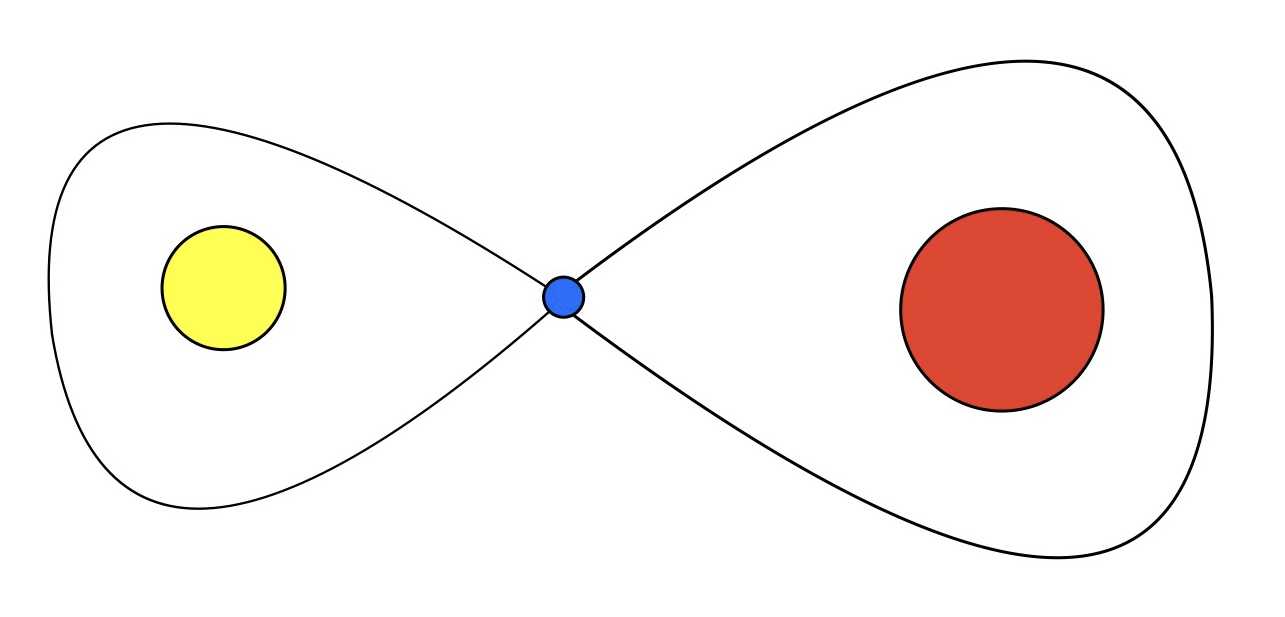
\includegraphics[width=0.5\textwidth]{Fig 1.jpeg}
    \caption{A model solar system with simplified orbits}
    \label{fig:orbit}
\end{figure}

Newton's Law of Gravitation states that, for any two masses $m_1$ and $m_2$ separated by a radius $r=|\bm{r_1}-\bm{r_2}|$ (where $\bm{r_1}$ and $\bm{r_2}$ are the positions of $m_1$ and $m_2$, respectively), the gravitational force of $m_2$ on $m_1$ is
\begin{equation}
    \bm{F_{12}}=-\frac{Gm_1 m_2}{|\bm{r_1}-\bm{r_2}|^3}*(\bm{r_1}-\bm{r_2})
\end{equation}
and the potential energy is
\begin{equation}
    U(\bm{r_1},\bm{r_2})=-\frac{Gm_1 m_2}{|\bm{r_1}-\bm{r_2}|}
\end{equation}
Since gravitation forces can be superimposed, the force of every body on a given body in an N-body system can be calculated as
\begin{equation}
    \bm{F_i}=\sum_{j=1, j \neq i}^N -\frac{Gm_im_j}{|\bm{r_i}-\bm{r_j}|}*(\bm{r_i}-\bm{r_j})
\end{equation}
Additionally, this is a closed system, so the total energy of the system is conserved.

\section{General Equations of Motion}
The given simplification of the problem into a one-body problem results (in the plane) in two degrees of freedom. In 3-dimensional space, there are three degrees of freedom. If the three masses initially lie in a plane together, they will remain in this plane. For simplicity, the initial conditions will be chosen for such a case.

Since the total energy of the system is preserved, and the potential of the system can be described as above, the following equations of energy hold
\begin{equation}
    T=\frac{1}{2}mv^2=\frac{1}{2}m(\dot{x}^2 + \dot{y}^2)
\end{equation}
\begin{equation}
    U_i=-\frac{Gmm_i}{|\bm{r_i}-\bm{r}|}
\end{equation}
\begin{equation}
    E=\frac{1}{2}m(\dot{x}^2 + \dot{y}^2)-\frac{Gmm_1}{|\bm{r_1}-\bm{r}|}-\frac{Gmm_2}{|\bm{r_2}-\bm{r}|}
\end{equation}
While solving a Lagrangian or Hamiltonian with these equations in cartesian coordinates is possible, simplifications arise when the system is converted to an elliptical coordinate system $(\xi,\eta)$ \ref{fig:coordinatesys}. If the masses are positioned in this coordinate system at the foci $2f$ apart, this is translatable to \[x=f\cosh{\xi}\cos{\eta}\] and \[y=f\sinh{\xi}\sin{\eta}\]
\begin{figure}
    \centering
    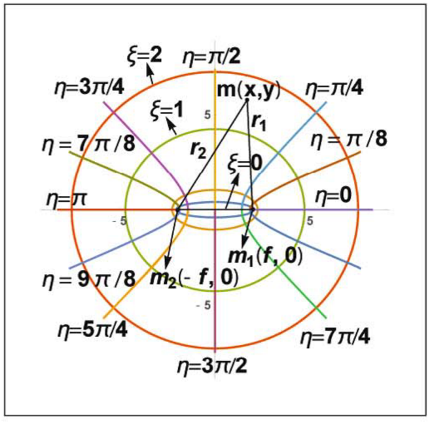
\includegraphics[width=0.5\textwidth]{Fig 2.png}
    \caption{the elliptical coordinate system $(\xi,\eta)$. $\xi$ can be thought of as correspondent to radial distance, and $\eta$ the angle.}
    \label{fig:coordinatesys}
\end{figure}
Therefore, there are two conserved quantities in the system: Whittaker's constant (see Krishnaswami 100) and total energy. Whittaker's constant can be represented as
\begin{equation}
    \begin{aligned}
        w=\bm{L_1}\cdot\bm{L_2}+2mf(-\mu _1 \cos{\theta _1} +\mu _2 \cos{\theta _2}) \\
        =m^2r_1^2r_2^2\dot{\theta _1}^2\dot{\theta _2}^2+2mf(-\mu _1 \cos{\theta _1} +\mu _2 \cos{\theta _2})\\
        =-2mf^2E-\alpha
    \end{aligned}
\end{equation}
where $r_i$ is the distance $|\bm{r_i}-\bm{r}|$ between $m_i$ and $m$; $\bm{L_i}=mr_i^2\dot{\theta _i}\hat{z}$ is the angular momentum of a mass; $\theta _i$ is the angle between $\bm{r_i}$ and the $x$-axis; $\mu _i=Gmm_i$; and $\alpha$ is the “separation constant” derived from the separation of variables of $E$ in elliptical coordinates (Krishnaswami 101 \cite{Krishnaswami2019}).

By using the Hamilton-Jacobi equation and Liouville's theorem, this system can be solved analytically. See Ó'Mathúna \cite{OMathuna2008} (pages 49-105 and 113-142) for a detailed solution.

\section{Numerical Solution}
While analytical solutions are useful for determining the exact motion of systems, numerical solutions are often much simpler. Such is the case here. Using Euler's approximation
\begin{equation}
    x(t+\delta t)=x(t)+\delta t\dot{x}(t)+O(\delta t^2)
    \label{eq:eulersmethod}
\end{equation}
and neglecting higher order terms $O(\delta t^2)$, the solution is quickly plottable in cartesian coordinates. This has error on the order of $\delta t$ (Wild 298 \cite{Wild1980}).

To do this, without loss of generality, shift the system so that $m_1$ is at the origin and $m_2$ is a distance d along the y axis from the origin. Now represent $m_2$ as a factor of $m_1=m_a$ such that $m_2=\alpha m_a$ \ref{fig:shiftedsys}.
\begin{figure}
    \centering
    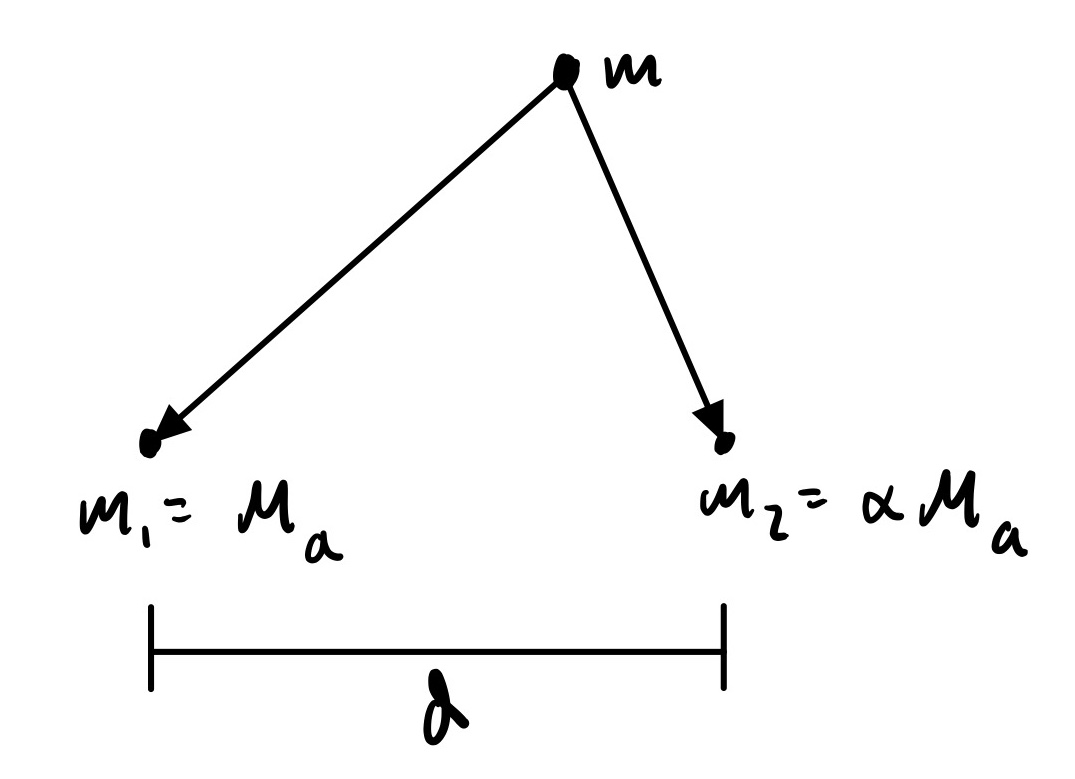
\includegraphics[width=0.5\textwidth]{Fig 3.jpeg}
    \caption{the shifted system with $m_1$ at the origin}
    \label{fig:shiftedsys}
\end{figure}

Up until this point, our masses and distances have been unitless and arbitrary. If these masses are instead measured in terms of solar units, further simplifications arise. If we set $m_a$ equal to a “solar mass”, we see that $Gm_a=4\pi^2$. This is because the angular velocity of a mass around a primary (for example, the Earth around the Sun) is $2\pi*AU/yr$, where $AU$ is the average distance between the primary and the mass.

Since we fixed the origin, our equations of motion now use relative positioning to the origin (and $m_1$). From this and Newton's Law of Gravitation, we see that
\begin{equation}
    F_x=-\frac{Gm_a m}{r_1^3}x-\frac{G\alpha m_a m}{r_2^3}(x-d)
    \label{eq:fx}
\end{equation}
\begin{equation}
    F_y=-\frac{Gm_a m}{r_1^3}y-\frac{G\alpha m_a m}{r_2^3}y
    \label{eq:fy}
\end{equation}
with $r_i=|\bm{r_i}-\bm{r}|$ the distance between $m$ and $m_i$. In cartesian coordinates, this results in
\begin{equation}
    \begin{aligned}
        \bm{r_1}=x\hat{x}+y\hat{y}\\
        \bm{r_2}=(x-d)\hat{x}+y\hat{y}
    \end{aligned}
\end{equation}
so
\begin{equation}
    \begin{aligned}
        r_1=\sqrt{x^2+y^2}\\
        r_2=\sqrt{(x-d)^2+y^2}
    \end{aligned}
\end{equation}

This is a system of nonlinear differential equations. As demonstrated above, analytical solutions are possible, but messy. Instead, using Euler's method \ref{eq:eulersmethod} and plugging in \ref{eq:fx} and \ref{eq:fy}
\begin{equation}
    \begin{aligned}
        \dot{x}(t+\delta t)=\dot{x}(t)+\delta t\ddot{x}(t)+O(\frac{\dot{x}}{dt^2})\\
        \approxeq\dot{x}(t)-\delta t4\pi^2(\frac{x}{r_1^3}+\frac{\alpha(x-d)}{r_2^3})
    \end{aligned}
\end{equation}
\begin{equation}
    \begin{aligned}
        \dot{y}(t+\delta t)=\dot{y}(t)+\delta t\ddot{y}(t)+O(\frac{\dot{y}}{dt^2})\\
        \approxeq\dot{y}(t)-\delta t4\pi^2y(\frac{1}{r_1^3}+\frac{1}{r_2^3})
    \end{aligned}
\end{equation}
If we set $f_n(t)=f(n\delta t)$, we get the following system of equations
\begin{equation}
    \begin{aligned}
        x_{n+1}=x_n+\dot{x}_n\delta t\\
        y_{n+1}=y_n+\dot{y}_n\delta t\\
        \dot{x}_{n+1}=\dot{x}_n-\delta t4\pi^2(\frac{x_{n+1}}{{r_1^3}_{n+1}}+\frac{\alpha(x_{n+1}-d)}{{r_2^3}_{n+1}})\\
        \dot{y}_{n+1}=\dot{y}_n-\delta t4\pi^2y_{n+1}(\frac{1}{{r_1^3}_{n+1}}+\frac{1}{{r_2^3}_{n+1}})
    \end{aligned}
\end{equation}
This is a programmable and plottable solution.

\section{Interpreting Solutions}
There are several cases in the limit where this solution demonstrates its clarity. The first case is when $d$ is very large (and $x$ is not). In this case, the terms dependent on $r_2$ disappear. This is equivalent to a system with only one star with mass $m_a$. On the other hand, if $d$ is very small, $r_1\approxeq r_2$. This is also equivalent to a system with one star, but this time the star has a mass $(1+\alpha)m_a$.

I have yet to finish my program, so I do not have plots of results to discuss. Once I do, I will analyze these plots, especially in terms of how varying different parameters results in different solutions, and how chaotic these parameters are.

Finally, I will demonstrate my code in the text and with a link to \href{https://github.com/jasperswallen/PHYS304-Project}{my public GitHub repository}
containing a Jupyter Notebook that readers will be able to download and run.

\appendix
\section{Code}
The code for this project is fully available at \href{https://github.com/jasperswallen/PHYS304-Project}{my public GitHub repository},
containing both a Jupyter Notebook and command-line Python script. The following is a stripped down version of \texttt{main.py}.

\begin{lstlisting}[language=Python, numbers=left, breaklines=true]
import matplotlib.pyplot as plt
import numpy as np
import math
### Input code is skipped for brevity
# declare arrays that will be appended to in loop
x = [moving_mass_x]
y = [moving_mass_y]
x_prime = [moving_mass_x_prime]
y_prime = [moving_mass_y_prime]

# We have the following equations of motion

for n in range(its):
    # calculate next x, y, x', and y'
    x_n_plus_one = x[n] + delta * x_prime[n]
    x.append(x_n_plus_one)
    y_n_plus_one = y[n] + delta * y_prime[n]
    y.append(y_n_plus_one)

    x_prime_n_plus_one = x_prime[n] - delta * 4 * (np.pi ** 2) * (x[n + 1] / np.power((x[n + 1] ** 2) + (y[n + 1] ** 2), 3 / 2) + alpha * (x[n+1] - mass_2_x) / np.power((x[n + 1] - mass_2_x) ** 2 + y[n + 1] ** 2, 3 / 2))
    x_prime.append(x_prime_n_plus_one)

    y_prime_n_plus_one = y_prime[n] - delta * 4 * (np.pi ** 2) * y[n + 1] * (1 / np.power((x[n + 1] ** 2) + (y[n + 1] ** 2), 3 / 2) + 1 / np.power((x[n + 1] - mass_2_x) ** 2 + y[n + 1] ** 2, 3 / 2))
    y_prime.append(y_prime_n_plus_one)

plt.plot(x, y)

masses = [[mass_1_x, mass_2_x, moving_mass_x],
          [mass_1_y, mass_2_y, moving_mass_y]]
colors = np.array([[255, 0, 0], [0, 255, 0], [0, 0, 255]])

plt.scatter(masses[0], masses[1], c=colors / 255)

labels = ["m1", "m2", "m"]
for i, txt in enumerate(labels):
    plt.annotate(txt, (masses[0][i], masses[1][i]))

plt.show()

\end{lstlisting}

\bibliography{bibliography}

\end{document}
